\section{Theorie}
Der Faraday-Effekt oder auch die Faraday-Rotation, beschreibt die Drehung der
Polarisationsebene eines Lichtstrahls beim Durchlaufen von Materie unter dem
Einfluss eines Magnetfeldes. Mit Hilfe des Effektes ist es möglich die
Bandstruktur in einem Halbleiter zu verstehen und die effektive Elektronenmasse
in diesem zu bestimmen.

\subsection{Das quantenmechanische Bändermodell}
Das quantenmechanische Bändermodell beschreibt das Energiespektrum eines
Elektrons in einem Kristall. Ein einzelnes Atom besitzt ein diskretes
Energiespektrum. Werden zwei Atome angenähert, sodass sie miteinander
wechselwirken, werdend die einzelnen Energieniveaus breiter. In einem Kristall
wechselwirken eine Mehrzahl von Atomen, sodass die Energieniveaus zu breiten
Bändern werden. Das Bändermodell eines Halbleiters wird in Abbildung
\ref{fig:band} dargestellt.

\begin{figure}[H]
  \centering
  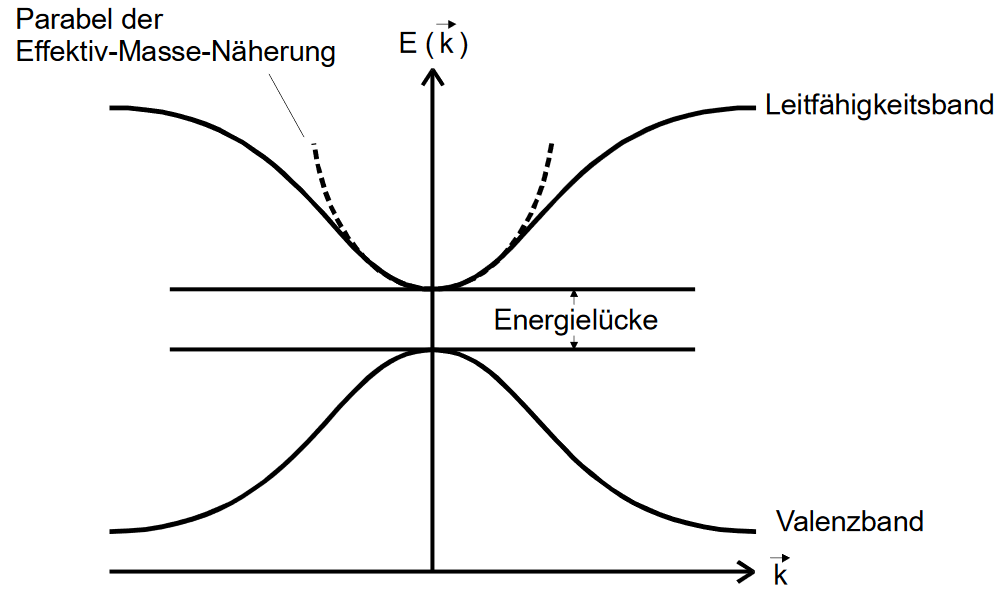
\includegraphics[width=13cm, height=7cm]{bandmodel.png}
  \caption{Vereinfachtes Bändermodell für einen Festkörper}
  \label{fig:band}
  \cite{skript}
\end{figure}

In dieser Abbildung werden die drei wichtigen Bereiche in einem Festkörper
dargestellt. Das Valenzband ist komplett mit Elektronen besetzt und trägt nicht
zur Leitfähigkeit eines Körpers bei. Das Leifähigkeitsband ist nicht
vollständig besetzt und ist somit für die Leitfähigkeit eines Festkörpers von
Bedeutung. Zwischen diesen Bereichen befindet sich eine Energielücke. Besitzt
die Energielücke eine Breite von über $\SI{10}{\electronvolt}$, so können die
Elektronen aus dem Valenzband selbst mit hinzugefügter Energie diese Lücke nicht
überwinden, der Körper ist somit ein Nichtleiter. Überlappen sich die beiden
Bänder, so wird der Festkörper als Leiterbezeichnet. Halbleiter besitzten eine
Energielücke, die die Elektronen nach hinzugefügter Energie noch überwinden
können. Daher stammt auch der Begriff des Halbleiters. Erst nachdem eine
gewisse Energie beispielsweise in Form von Wärme hinzugefügt wird, können die
Elektronen die Lücke überwinden und der Körper leitet. Wird keine Energie
hinzugefügt, befinden sich die Elektronen im Valenzband in einer festen Bindung
und können die Lücke nicht überwinden, der Stoff ist somit nicht leitend.

\subsection{Die effektive Masse}
